\chapter[Short name of chapter]{This is the very long name of the first chapter. It is too long.}

{\color{lmpsblue} \epigraph{La LATIN-PGD c'est génial !}{Alexandre Daby-Seesaram}}

\begin{chapabstract}
    This is the chapter abstract. You can customize its style by modifying the environment \texttt{chapabstract} in the \texttt{lmpsthesis.cls} file.
    \lipsum[1]
\end{chapabstract}

\minitoc

\section{Presentation of the template}%
\label{sec:presentation_of_the_template}

\subsection{An equation}%
\label{sub:an_equation}

This subsection contains the equation of the harmonic decomposition of an elasticity tensor,
\begin{equation}\label{eq:harmonic_decomposition}
    \ela =
        2 \mu \J +
        \kappa \id{2} \otimes \id{2} +
        \frac{1}{2} (\id{2} \otimes \dev{\dil} + \dev{\dil} \otimes \id{2}) +
        \har
\end{equation}
where
    $\mu$ is the shear modulus,
    $\kappa$ is the bulk modulus,
    $\dev{\dil}$ is the deviatoric part of the dilatation tensor, and
    $\har$ is the harmonic part.
Moreover, $\id{2}$ is the second order identity tensor and $\J$ is the deviatoric projector.
You can refer to this equation using the package \texttt{cleveref}\footnote{Guide to \texttt{cleveref}: \url{https://texblog.org/2013/05/06/cleveref-a-clever-way-to-reference-in-latex/}.}.
The \cref{eq:harmonic_decomposition} contains the harmonic decomposition.
\begin{remark}
    The \cref{eq:harmonic_decomposition} uses notations defined in the List of Symbols in the frontmatter.
    Those notations are defined using custom commands in the \texttt{notations.tex} file.
\end{remark}

\subsection{Adding figures}%
\label{sub:adding_figures}

\paragraph{Paragraph with a figure}%
\label{par:paragraph_with_a_figure}
You can insert figures and easily refer to them.
For instance, \cref{fig:c1_cracking_pattern} contains a cracking pattern generated with the \emph{beam-particle} model in the code \texttt{DEAP}.
\begin{figure}
    \centering
    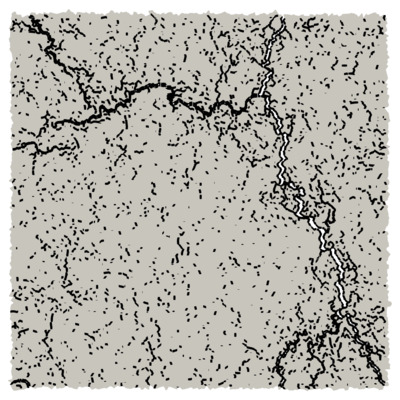
\includegraphics[width=0.3\textwidth]{figures/chapter_1/cracking_pattern_pbc_willam_4.jpg}
    \caption{This is a cracking pattern from DEAP. This file has been compressed to be as small a possible.}
    \label{fig:c1_cracking_pattern}
\end{figure}
We recommend placing images files inside the \texttt{figures} directory.
As you can have a lot of figures, we also recommend making a subdirectory for each chapter.

\paragraph{Paragraph with a tikzpicture}%
\label{par:paragraph_with_a_tikzpicture}
You can also add figures using Tikz.
To use Tikz and PGFPlots in this template, you must activate the option \texttt{tikz} in the definition of the document at the beginning of the file \texttt{PhD\_Thesis.tex}.
\Cref{fig:c1_illustrations_symmetry_classes} contains an illustration of the symmetry classes of elasticity tensors in 2D using Tikz.
\begin{figure}
    \centering
    \tikzsetnextfilename{c1_illustrations_symmetry_classes}
    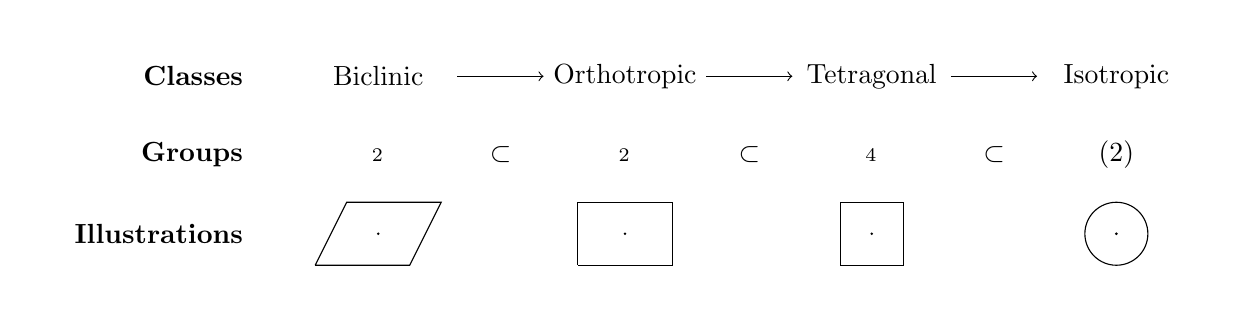
\begin{tikzpicture}[
        header/.style={align=right, minimum height=1cm, text width=2.5cm},
        cell/.style={align=center, minimum height=2em, minimum width=2cm},
    ]
    % Create a matrix
    \matrix [column sep=0.3cm] {
        % Symmetry classes
        \node[header] {\textbf{Classes}};  &
        &
        \node[cell] (bic) {Biclinic};               &
                                                    &
        \node[cell] (ort) {Orthotropic};            &
                                                    &
        \node[cell] (cub) {Tetragonal};             &
                                                    &
        \node[cell] (iso) {Isotropic};              \\
        % Groups
        \node[header] {\textbf{Groups}};            &
        &
        \node[cell] (zz2) {$\ZZ_2$};                &
        \node {$\subset$};                          &
        \node[cell] (dd2) {$\DD_2$};                &
        \node {$\subset$};                          &
        \node[cell] (dd4) {$\DD_4$};                &
        \node {$\subset$};                          &
        \node[cell] (oo2) {$\OO(2)$};               \\
        % Geometric figures
        \node[header] {\textbf{Illustrations}}; &
        &
        \fill[black] (0,0) circle (0.5pt); \draw (-0.6-0.2,-0.4) -- (-0.6+0.2,0.4) -- (0.6+0.2,0.4) -- (0.6-0.2,-0.4) -- (-0.6-0.2,-0.4);  &
        &
        \fill[black] (0,0) circle (0.5pt); \draw (-0.6,-0.4) -- (-0.6,0.4) -- (0.6,0.4) -- (0.6,-0.4) -- (-0.6,-0.4);  &
        &
        \fill[black] (0,0) circle (0.5pt); \draw (-0.4,-0.4) -- (-0.4,0.4) -- (0.4,0.4) -- (0.4,-0.4) -- (-0.4,-0.4);  &
        &
        \fill[black] (0,0) circle (0.5pt); \draw (0,0) circle (0.4);                                                 \\
    };
    % Add paths
    \draw[->] (bic) -- (ort);
    \draw[->] (ort) -- (cub);
    \draw[->] (cub) -- (iso);
\end{tikzpicture}

    \caption{A tikz illustration of Symmetry classes and their representative group for 2D elasticity tensors. The illustrations are geometric figures in R2 representative of each of the symmetry classes.}
    \label{fig:c1_illustrations_symmetry_classes}
\end{figure}
\begin{remark}
    If you don't want to use Tikz, you should deactivate the option in the document class at the beginning of the main file.
\end{remark}

\begin{remark}
    Note that \texttt{tikzpicture} is automatically externalized.
    To avoid any issues, we recommend you to name the \texttt{tikzpicture} using the command \texttt{\textbackslash textsetnextfilename}.
\end{remark}


\section{Doing some bibliography}%
\label{sec:doing_some_bibliography}

\paragraph{Citing papers}%
\label{par:Citing papers}
Using \texttt{biblatex}, you can cite different works.
Here is an example with different thesis using the early version of this template, such as \textcite{cherriere_elaboration_2023,caruel_caracterisation_2023,ruda_methode_2023,abdel_hafiz_etude_2023}, and more recent version of this template \parencite{daby-seesaram_towards_2023,loiseau_formulation_2023}.
Here, you can also cite some articles.
For instance, you can refer to the works of \textcite{wurtzer_premiere_2022,ribeiro_nogueira_differential_2024}.
You can also cite paper in parentheses \parencite{ruda_first_2022,daby-seesaram_hybrid_2023}.
The list of references appears at the very end of the document.

\section{Another section}%
\label{sec:Another section}

\subsection{With a first subsection}%
\label{sub:with_a_first_subsection}

\lipsum[2-4]

\subsection{And a second subsection}%
\label{sub:and_a_second_subsection}

\lipsum[2-4]

\begin{chaptersummary}
    \lipsum
\end{chaptersummary}
